
In this chapter, I show how we extend our engine to support
verification of concurrent programs with fine grained locking.
As illustrated in Chapter \ref{chapter:driver}, our definition of
certified abstraction layers do not directly work with concurrent programs,
as the contextual refinement between the specification and implementation
would not hold due to the arbitrary interleaved executions with other
devices/CPUs. This is because the way we specify the function
does not take account the potential change to the (shared) abstract states
and memory due to the interleavings. On the other hand, it is definitely
not practical to encode all possible ways of the state changes from
interleaved executions in the specifications themselves.

Thus, we need a way to effectively represent the shared states among programs
on different CPUs, and the non-deterministic accesses to these shared
states. We would also want to reuse all the techniques
that we have built for verification of sequential programs.
Recall that we have successfully handled some limited form of concurrency
between the devices and a sequential program in Chapter \ref{chapter:driver}.
There, we have developed a new machine model, where the devices are treated
as if they do not execute together with the CPU, and only try to replay
the states of a device when we disable and enable the interrupts on that
device. These two are considered as valid synchronization points because
we do not access the states of the device when the interrupt of the device
is enabled, and we can recompute the current states of the device solely by
applying the device model to the list of external events we observe on that device.

This is clearly restricted to the limited form of concurrency in consideration,
and cannot be directly applied to reasoning of arbitrary concurrent program.
Yet, the general idea is still valid, and we have indeed extended this line of
idea to a concrete framework that is suitable to reason about arbitrary
concurrent programs with fine grained locking in modular ways.
By modular reasoning of concurrent programs, we would expect to reason about
each program running on a CPU or thread separately, by making valid assumptions
to the rest of programs and outside world, and in the end link these individual
proofs formally to reach a final conclusion about the entire program when they
run altogether concurrently. 
In Chapter \ref{chapter:driver}, we still use the abstract states
to model the shared states (the states of devices), which, at synchronization
points, get computed by applying the effect of external events on the current
shared states. Naively applying this would cause the discrepancy when the current
thread uses the abstract states to represent the shares states, while the rest
of the world uses the events. Instead, we always use the list of events to represent
the shared states among threads and processes. In this model, modifying shared
states can be specified simply as appending a new corresponding event to the
event list, and this list can be synchronized by appending the list of events
generated by the rest of the world at every carefully chosen synchronization points.
The the actual shared states can be derived from the list of events by replaying
the effects of the each event in the list from an initial state. We attach such
\emph{replay function} for each shared state and related events.

Recall that in the sequential world, the task of layer based verification is to prove
the contextual refinement between the concrete function implementation manipulating
concrete in-memory data and the abstract high level specification described in
terms of the corresponding abstract states. In this case, the context would be the
user program, other kernel or hypervisor functions, {\it etc}.
In the concurrent world, we also have the programs running on other CPUs/threads,
in parallel with the current function being verified.
Thus, in this case, the task involves proving the contextual refinement between
the function implementation operating on the shared memory and abstract states,
and the abstract high level atomic specification that triggers an atomic high level
event. In the next section, we present this new framework in more detail.

\section{Certified Concurrent Abstraction Layers}

\paragraph{Machine State}
Our new x86 machine state $s$ is a tuple $s~:=~(c, f_p, m, a, l)$.
Here, the component $c$ stands for the current CPU ID, and $f_p$ is
a partial map from a CPU ID to the private states of that CPU.
In addition, $m$ stands for the memory shared across CPUs, and $a$
stands for the shared abstract states. The list $l$ represents
the list of observable global events in the chronological order.
As we mentioned earlier, we represent all shared
states by the list of events, where the concrete states can be reproduced
by applying the replay function to the list of events starting from the initial states.

\paragraph{Transitions}
In the new concurrent machine, a transition may refer to a regular execution
of an assembly instruction, invocation of a private primitive that only changes
CPU local states, or a shared primitive call that could trigger events
observable to other CPUs. To model the non-deterministic execution among
different CPUs, we also have a special transition that changes the current
CPU ID $c$ to some other CPU ID, which we call \emph{hardware scheduling transition}.


\paragraph{Restrictive Memory Model}
Eventually, we would like to prove that every memory access from our entire
verified concurrent program is safe, and there is no data race.
Instead of proving all these desired memory access properties as separate
lemmas for every program, as our usual verification technique, we take a
more systematic approach, i.e., we design a memory model only for safe
memory access such that all the undesired programs semantically get stuck
on our memory model. This ensures that every verified program on our framework
must be data race free.

As a result, in our memory model, we associate every memory block $b$ with
an ownership status in the abstract state $a$, which can only be manipulated
by two new logical abstract primitives \emph{push} and \emph{pull}.
The \emph{pull} operation modifies the ownership status of the memory block
from ``free'' to ``owned by $c$'', while the \emph{push} operation frees back
the ownership of the memory block, together with the updated memory.
These two operations abstract all shared memory access at our
lowest machine model as atomic logical primitives that triggers corresponding
\emph{push} and \emph{pull} events. 
As described above, if a program tries to pull a non-free location, or tries to
access or push to a location that is not owned by the current CPU, the
machine semantics gets stuck. 
This way, we encapsulate every valid shared memory access with corresponding
\emph{push} and \emph{pull} events from involved CPUs.
We show in Section \ref{veri-ticket-lock}
how we can further encapsulate and abstract these logical primitives to
build a spinlock module.


\paragraph{Active CPU Set and Environmental Context}
To enable modular reasoning of concurrent programs, we would like a way
to semantically reason about only part of the whole program locally, by
making reasonable assumptions on the rest of programs, and finally formally
combine the reasoning of these individual programs together, to reach a
final conclusion about the full program.
We call the set of CPUs in consideration the \emph{active CPU set} $A$, and
specify the assumptions over the external world outside $A$ as the
environmental context $\oracle$, which is a partial map from a list of
current global event log $l$ to another list of events $l'$ that corresponds
to the list of observable events triggered by the CPUs outside $A$ at this
interleaving point. We denote such concurrent layer interface $L$ parameterized by
an active CPU set $A$ and environmental context $\oracle$ as
$\PLayer{L}{A}{\oracle}$.

We encode our assumptions on the external world by
enforcing a \emph{Rely} condition on the list of event logs
the environmental context returns,
and represent our own invariants by introducing a \emph{Guarantee} condition
on the list of events triggered by programs running on the active CPU set $A$.
If we have separately verified two sets of concurrent programs running on
a disjoint sets of CPUs $A$ and $B$, and each of the \emph{Guarantee} condition
implies the other's \emph{Rely} condition, then we can merge these two proofs
together to derive a proof on a combined concurrent program running on the
active CPU set $S_{AB}=A\cup B$ and the environmental context 
$\oracle_{AB}=\oracle_A\cap\oracle_B$.
Since the event list $l$ is part of our abstract state, and the list of events
from the environmental context is also appended to $l$, both the \emph{Rely}
and \emph{Guarantee} condition can be represented as regular layer invariants
in our concurrent certified abstraction layer framework.

\ignore{
\paragraph{Concurrent Layer Interface}

Now we define the \emph{concurrent layer interface} $\PLayer{L}{A}{\oracle}$,
parameterized over the active CPU set $A$, and the environmental context
$\oracle$, as a tuple $(\Layer, \Rely, \Guard)$, where the $\Layer$ defines
the abstract states and primitives (similar to the sequential version),
and $\Rely$ and $\Guard$ being the \emph{Rely} and \emph{Guarantee} condition.
}

\paragraph{Building Concurrent Certified Abstraction Layers}
Now we define the contextual refinement in the concurrent setting,
using the definition in the sequential case.

\begin{definition}[Contextual Refinement]
For every code module $M$, active CPU set $A$, and environmental context
$\oracle$, we say $\llbracket{}M\rrbracket{}L_1$ contextually refines
$L_2$ over $A$ and $\oracle$ if and only if there exists a function
$f$ such that $\llbracket{}M\rrbracket{}\PLayer{L_1}{A}{\oracle}$ contextually
refines $\PLayer{L_2}{A}{f(\oracle)}$. 
\end{definition}

Similar to the sequential case, we have developed some proof patterns on
building concurrent certified abstraction layers, layer by layer.
Our verification is still per function basis, and we verify the programs
running on each CPU separately, and build up the standard layer hierarchy
$\PLayer{L}{\{c\}}{\oracle}$ for each CPU $c$. For simplicity, we note this
\emph{CPU local layer} as $\PLayer{L}{c}{\oracle}$.
In the end, we compose these proofs for each CPU
into a combined proof for the whole concurrent program.

We have developed two proof patterns to help building certified concurrent
abstraction layers. First, we use \emph{fun-lift} pattern to abstract shared
physical memory into shared abstract states, and specify and verify the
concurrent functions with these abstract states, in a way very similar to
how we build the sequential layers. Note that this process does not change
any potential interleavings in the programming executions, and each shared
operation is specified by querying the environmental context to obtain the
external event list at every interleaving point, i.e., our primitive specifications
are no longer atomic as their behavior depends on other concurrent programs' behavior
in the middle of the primitive executions. On the other hand, by not handling
the concurrency at this level allows us to be able to reuse most of the
frameworks and techniques we have built for verifying sequential programs.

Once we are at a layer where we have a full behavior of the shared
``atomic'' primitives, we utilize the second \emph{log-lift} pattern to
lift the layer into a new layer where the specifications of the shared
primitives are atomic, i.e., they simply trigger a new single atomic
event. Proving the contextual refinement between these two layers include
the critical concurrency reasoning on the fact that the events can be
shuffled and merged into a new list where we can always map a consecutive
list of underlay events into a single new event at the overlay.
Concretely, we need to find a function $f$ that can transform the environmental
contextual of underlay into one at overlay, and a refinement relation $R$
that matches the underlay and overlay states, especially the two event list
with events generated both locally and returned by the environmental context.
We illustrate this process in more details in the examples in subsequent sections.

\paragraph{Multicore Linking Theorem.}
By composing all the CPUs in the machine (denoted as the set $D$), the resulting 
layer interface does not depend on any environmental events except those
hardware scheduling transitions among different CPUs.
We construct such a layer interface $\PBoot[D]$
using the primitives provided by the layer $\Mach_{\boot}$, which is the lowest
layer that we use to model the multicore hardware environment. 
We can then prove a contextual refinement from  $\Mach_{\boot}$ to $\PBoot[D]$
for every possible interleaved executions.
\begin{theorem}[Multicore Linking]
\label{thm:link}
$\forall P, \sem{\Mach_{\boot}}{P} \refines_R \sem{\PBoot[D]}{P}$
\end{theorem}
This theorem ensures that all code verification over $\PBoot[D]$ can be propagated down to the x86 multicore hardware 
$\Mach_{\boot}$.


\section{Verification of Ticket Lock}
\label{veri-ticket-lock}

\begin{figure}[t]
\lstinputlisting [language = C] {src/ticket_lock.c}
\caption{Pseudocode of ticket lock implementation.}
\label{fig:ticket_lock_c}
\end{figure}

\begin{figure}
	\lstinputlisting [language=Coq] {src/ticket_lock.v}
	\caption{Specifications of ticket lock acquire and release functions}
	\label{fig:ticket_lock_v}
\end{figure}

Spinlocks are one of the most basic synchronization
methods for multicore machines; they are used as building
blocks for shared objects and more sophisticated synchronizations.


A spinlock enforces mutual exclusion by restricting CPU access to
a memory location $b$. Lock operations can be viewed
as ``safe'' versions of $\push/\pull$ primitives.
For example, when the lock acquire  for $b$ succeeds,
the corresponding shared memory is guaranteed
to be ``clean'', meaning that it is safe to 
pull the contents to the local copy at this point.
As an example, Fig.~\ref{fig:ticket_lock_c} shows
an implementation of the ticket lock algorithm \cite{mcs91}.
As can be seen in Fig.~\ref{fig:ticket_lock_c},
the $\acq/\rel$ functions invoke the $\push/\pull$ primitives.
\footnote{Note that even though these primitives are
called in the layer as if they are actual function primitives,
those are only logical primitives that do not intend to incur
any performance overhead, and are only used as a verification
technique.}

The ultimate atomic specifications for the lock acquire and release primitives
are shown in Figure \ref{fig:ticket_lock_v}. 
Here, as a synchronization point, \textsf{acquire\_lock\_spec} first queries the
environmental context to obtain the list of environmental events to sync, adds
them to the event list, together with its single \textsf{E\_ACQ\_LOCK} event.
Meanwhile, \textsf{release\_lock\_spec} is very similar, except it adds its
 \textsf{E\_REL\_LOCK} event instead to the event list. \footnote{As shown in the figure,
 the events are prepended instead of appended in the end of the list, because it is easier
 to work with, based on the implementation of the list in Coq.}
The atomicity is implied from the fact
that the primitive attaches a single \textsf{E\_ACQ\_LOCK} or \textsf{E\_REL\_LOCK}
event to the event list, thus would not be able to have any other observable event
injected in the middle. 

Next, we present how we manage to verify the implementation shown in Figure
\ref{fig:ticket_lock_c} satisfies the atomic specifications shown in Figure
\ref{fig:ticket_lock_v}. As we can observe, the gap between the two is reasonably
big and there seem not be a direct connection between the two.
Following our mantra, we achieve the verification across multiple abstraction layers,
such that we can focus merely on the functional verification when we deal with the
C code reusing all the technologies we have developed so far for our automation engine,
and separately deal with all other proof aspects at logical level.

\paragraph{Layer Interface TicketLockIntro}
As usual, we introduce a new layer interface TicketLockIntro to perform data
abstraction and turn the concrete in memory ticket lock
data structure into logical mappings of abstract ticket lock indexed by the block,
and provided the \textsf{get\_now}, \textsf{inc\_now}, and \textsf{FAI\_ticket}
primitives, as shown in Figure \ref{fig:ticket_lock_c}. They all have atomic specifications
where they each appends a corresponding low level event to the event list.
The list of events generated by the primitives in TicketLockIntro are
\textsf{E\_INC\_TICKET cpu b}, \textsf{E\_INC\_NOW cpu b}, \textsf{E\_GET\_NOW cpu b}, 
\textsf{E\_PULL cpu b} and \textsf{E\_PUSH cpu b bl}.

TicketLockIntro also provides a replay function \textsf{ReplayTicket} which takes the
list of the generated events for the block, and reconstruct the value of \textsf{ticket} and
\textsf{now}. The definition is as one would expect: it increments the \textsf{ticket} and
\textsf{now} field when it sees the \textsf{E\_INC\_TICKET} and \textsf{E\_INC\_NOW}
event respectively, and ignores all other events. This replay function is used, for example,
in the specification of \textsf{get\_now} to return the current \textsf{now} field.


\paragraph{Layer Interface TicketLockOp}

Next, we perform the actual verification of the function \text{acq\_lock} and \textsf{rel\_lock}.
Instead of directly verifying them against their atomic specification shown in Figure
\ref{fig:ticket_lock_v}, we first utilize \emph{fun-lift}, and verify the code against
intermediate specifications we came up where the specifications contain the exact same
interleaved execution sequence such that we no longer need to reason about
any potentially interleavings in the programming executions during code verification.

To illustrate the process better, we give details on the verification of the \textsf{acq\_lock}
function. As shown in Figure \ref{fig:ticket_lock_c}, the implementation of \textsf{acq\_lock}
contains a ``potentially infinite'' loop, where the function loops until the \textsf{now} field
of the ticket becomes the same as its own ticket number in hand.
The reason why this function would always terminate involves in the proof of the starvation-freedom
of this lock implementation where we need to also reason about the scheduler implementation and
thread contexts. As always, we would like to split out reasoning of these aspect from the actual
code verification, and separately perform this proof afterwards at a more suitable logical level.

Our usual approach on separating complex logical reasoning out of code proof is to have an intermediate
logical specification that is very similar to the implementation. Similarly, we have designed an auxiliary predicate
\textsf{WaitTicket} that mimics the loop in the code, where it repeatedly generates the \textsf{E\_GET\_NOW}
event until the \textsf{now} field becomes the same as the provided ticket number. 
On the other hand, we cannot have a specification that potentially does not terminate.
Thus, \textsf{WaitTicket} also takes an integer \text{bound} which acts as the upper bounce on the
number of times \textsf{WaitTicket} can loop, and it gets stuck if the \textsf{now} field
does not reach its ticket number within the bound.
The definition of \textsf{WaitTicket} is shown in Figure \ref{fig:wait_ticket_v}.

The intermediate specification defined using \textsf{WaitTicket} is shown in Figure \ref{fig:acq_lock_concrete_v}.
Here, it first synchronizes its event list by querying the environmental context, adds the
\textsf{E\_INC\_TICKET} event to the list (corresponding to the call to \textsf{FAI\_ticket} in the code),
grabs the current ticket and number, and waits for the turn using the \textsf{WaitTicket} predicate
with the specified bound, and finally adds the event \textsf{E\_PULL} (for the call to \textsf{pull}).
Recall that we verify the forward simulation, thus our code verification lemma is always stated
in a way such that if the specification does not get stuck, then the code terminates and reaches
the same states and return value. Thus, the fact that the \textsf{acquire\_lock\_intermediate\_spec}
does not get stuck would imply that the provided upper bound is large enough to get back to
the current CPU's turn. We would need to separately prove that there exists a very large bound
such that the specification never gets tuck (proof of starvation-freedom). We get back to this proof later
in this section.

\begin{figure}
	\lstinputlisting [language=Coq] {src/wait_ticket.v}
	\caption{Predicate WaitTicket}
	\label{fig:wait_ticket_v}
\end{figure}

\begin{figure}
	\lstinputlisting [language=Coq] {src/acq_lock_concrete.v}
	\caption{Intermediate specification of acquire lock function}
	\label{fig:acq_lock_concrete_v}
\end{figure}

There is still one discrepancy between the \textsf{acquire\_lock\_intermediate\_spec} and the
implementation. In order to facilitate the refinement proof between the intermediate specification
and the corresponding atomic specification, our ticket replay function \textsf{ReplayTicket}
uses integers to represent the \textsf{ticket} and \textsf{now} field that increments indefinitely.
On the other hand, our C implementation uses finite precision integers that wraps back to zero when
we increment from its maximum value. That is why we use the $!=$ operator instead
of $<=$ in Figure \ref{fig:ticket_lock_c}.
Again, to split out the reasoning of finite precision integer mappings, we use a separate
replay function \textsf{ReplayTicketWraparound} in the \textit{low level specification} of
\textsf{acq\_lock} that is used against the code verification, which also wraps the \textsf{ticket}
and \textsf{now} fields back to zero when they reach their maximum.
Then we separately perform the mapping between
the finite and infinite precision integers during the refinement proof. This way, we no longer
need to worry about the mapping repeatedly during the intermediate code proofs. During
the forward simulation refinement proof, this proof can be performed once and for all by
simply mapping the numbers from high level specifications into their wrapped versions
in the low level specifications.

Next, we show how we perform the actual functional verification using our automation engine
against the low level specification, which is already extremely close to the implementation.
The major challenge here is to get the proper loop invariant to prove the termination of the while
loop. Before we present the loop invariant, we first show the list of lemmas we have developed
to assist the loop invariant preservation proof, listed in Figure \ref{fig:acq_lock_lemmas_v}.

\begin{figure}
	\lstinputlisting [language=Coq] {src/acq_lock_lemmas.v}
	\caption{Lemmas for proving acquire lock}
	\label{fig:acq_lock_lemmas_v}
\end{figure}

Here, \textsf{WaitTicketWraparound} is a predicate similar to \textsf{WaitTicket} except it uses
\textsf{ReplayTicketWraparound} instead of \textsf{ReplayTicket}.
Note the predicate \textsf{WaitTicketWraparound} gets stuck when the bound is not sufficiently large.
On the other hand, we know the provided bound is large enough as we know the specification does
not get stuck in the precondition. Thus, we would need to repeatedly prove that \textsf{WaitTicketWraparound}
does not get stuck while we verify the loop. Instead, as define another predicate
\textsf{WaitTicketWraparoundSafe} where it returns the current event list when the counter gets down
to zero, instead of getting stuck. We use this definition instead for verification of the loop, as this
predicate never gets stuck by definition, and returns the same list when the bound is sufficiently large (which
we know it is). The lemma \textsf{WaitTicketWraparoundStops} shown in Figure \ref{fig:acq_lock_lemmas_v}
is used in the end to convert our post condition back into the one using the proper \textsf{WaitTicketWraparound}.
It states that if we could wait for our turn with sufficiently large bound, then there should be a least
upper bound no bigger than the current bound that both original and safe versions would lead to the same event list.
The lemma \textsf{WaitTicketWraparoundImpliesSafe} shows that for a valid bound, both the original
and safe versions return the same list, and the lemma \textsf{WaitTicketWraparoundSafeInv}
presents the inversion principle for the predicate \textsf{WaitTicketWraparoundSafe}.
Finally, the lemmas \textsf{WaitTicketWraparoundSafeNeq} and \textsf{WaitTicketWraparoundEq}
describe the situation when we have short or large bound, respectively.

Let the integer $K$ indicate the smallest bound that would allow the \textsf{WaitTicketWraparound}
to reach its own turn (not to get stuck). We know such $K$ exist from the precondition that the specification
of \textsf{acquire\_lock\_intermediate\_spec} does not get stuck. Then we can specify
our loop invariant in the following way. 

\begin{definition}[Loop Invariant for \textsf{acq\_lock}]
There exists integers \textsf{loopCounter} and \textsf{newNow} such that
\begin{itemize}
\item the \textsf{now} field in the new abstract state $\textsf{adt}'$ is \textsf{newNow} when replayed from the log,
\item $\textsf{adt}' = \textsf{adt}~\{\textsf{event\_log}: \textsf{ZMap.set b (ObservableEvents l') (event\_log adt)}\}$,


where $l' = \textsf{WaitTicketWraparound}(\textsf{loopCounter cpu b ticket (event\_log adt)}$,
\item either $0\le \textsf{loopCounter}<K$ and $\textsf{newNow}\neq\textsf{ticket}$ or
$\textsf{loopCounter}=K$ and $\textsf{newNow}=\textsf{ticket}$.
\end{itemize}
\end{definition}

\begin{definition}[Termination Metric] $K - \textsf{loopCounter}$.
\end{definition}

The fact that the new abstract state $\textsf{adt}'$ after one loop iteration have to be the same as
waiting with the current loop counter would infer that the next loop counter is one greater than the current
loop counter, thus we can derive the termination in addition with above monotonically decreasing termination
metric.
With this loop invariant and termination metric, together with the lemmas for verifying the loop body,
we can discharge the remaining proofs with our automation engine. 

Next, we tackle one last remaining proof obligation, i.e., to find out a sufficiently large bound
that would never let the intermediate acquire lock specification get stuck.
This is necessary because we eventually need a specification which does not take a bound
as argument, as the user would never be able to explicitly give us the bound.
To prove that such number exists, we make following two assumptions. 
First, the hardware scheduling transition
is fair, i.e., there exists a number $h$ such that the nondeterministic execution is
guaranteed to get back to the previous CPU within $h$ hardware steps.
Second, every CPU who acquires the ticket lock releases the lock within
$r$ steps for some constant $r$. This is also a reasonable assumption because if someone
holding the lock never releases the lock, no one else can ever obtain the lock
again. Both of these assumptions are formally enforced by introducing
them as layer invariants on the event list $l$.
Given these two assumptions, and also assuming there are $n$ number
of CPUs available on the machine, we can conclude that each CPU
needs to wait on the lock for at most $h * r * n$ steps, as even if all
other CPUs were in the queue ahead of the current CPU, they would eventually
all release the lock within these many steps and no one can take the lock
bypassing the currently CPU's turn by definition of the ticket lock.

This is one of the typical example where complex logic is involved in reasoning about correctness
of a very simple and short piece of C code, which involves significantly larger number of proof
scripts than the actual source code. Yet, by carefully tackling various challenges in isolation, we
can still manage to verify the ticket lock implementation relatively easily using our automation engine.

\paragraph{Layer Interface TicketLock}

Finally, we introduce a new layer interface where the lock acquire and release
primitives have the atomic specifications as shown in Figure \ref{fig:ticket_lock_v}.
At TicketLock, we no longer have any of the low level events shown in previous
layer interfaces, but two new events \textsf{E\_ACQ\_LOCK} and \textsf{e\_REL\_LOCK},
generated by the two new lock primitives (see Figure \ref{fig:ticket_lock_v}).

In order to prove the contextual refinement between TicketLockOp and
TicketLock layers, we need to find a function $f$ that converts
one environmental context into the other, and also a refinement relation
$R$ that related the list of events in two layers.
We map two list of events by mapping \textsf{E\_PULL} in 
TicketLockOp to \textsf{E\_ACQ\_LOCK} in TicketLock,
and \textsf{E\_INC\_NOW} to  \textsf{E\_REL\_LOCK}, respectively, ignoring all other
events in TicketLockOp. Function $f$ can be derived from this relation by
first applying the underlay environmental context in underlay event list,
and convert the list into the list of overlay events following the same conversion
rule as in the refinement relation.
Then we finally prove that the refinement relation is preserved for every primitive
over this setting.
This simulation proof is only between specifications, and in the end,
we can compose proofs of individual primitives to derive the full
contextual refinement as in the sequential case.

\paragraph{Extending to Other Type of Spinlocks}
This event-based specification for the spinlock is general enough
to capture  other implementations like the \emph{MCS Lock},
which is known to have better scalability than ticket lock
over machines with a larger number of CPUs. We have also
implemented a version of MCS locks~\cite{kim2017safety}, following
similar proof technique, while maintaining exactly same high level
specifications for $\acq$ and $\rel$ as in $L_3$ above.


\section{Shared Queue Object}

\begin{figure}[t]
\lstinputlisting [language = C, multicols=2] {src/dequeue.c}
\caption{Pseudocode of dequeue implementation.}
\label{fig:exp:dequeue}
\end{figure}

Given that we have verified ``atomic'' lock acquire and release primitives,
we can utilize these spinlocks to verify more useful concurrent
data structures and programs. Shared queue is one of the widely used
data structures used in concurrent programs like producer/consumer,
scheduler, {\it etc}. 

The specification of a shared queue object should provide a high level abstract
interface by hiding all the low level details,
to ease the verification of programs using the object.
However, the large gap between this high level abstract specification
and the low level efficient implementation makes the verification of the shared queue object
itself extremely challenging.
The previous verification technique for shared queue object~\cite{lili16}
has to inline the lock implementation and duplicate the lock-related proofs, due
to the lack of modular layered approach.

Figure \ref{fig:exp:dequeue} shows the implementation of dequeue operation, where
we represent the queue in terms of a doubly linked list. 
As shown in the figure, we utilize an auxiliary function $\deq\comm{\_t}$ which
performs the actual operations on the queue. The main function $\deq$ simply
wraps $\deq\comm{\_t}$ with the lock acquire and release functions.
To verify this shared queue, we first verify the $\deq\comm{\_t}$ function
via the  \emph{fun-lift} pattern for sequential program, where the specification
assumes that the lock is already held, thus no interleaved executions are possible
in the middle of $\deq\comm{\_t}$. 
This way, we can reuse the verified sequential queue with minimum change.
Then we utilize 
the \emph{log-lift} pattern to introduce another layer for the main $\deq$ function
where it simply generate one single $\deq$ event. This can be done by merging two
queue-related lock acquire and release events underlay into a single $\deq$ event
at the overlay. 


\section{Supporting Multiple Virtual Machines}

Given that we can reason about concurrent programs, we have extend the OS kernel
presented in Chapter \ref{chapter:sequential} into a concurrent kernel that can boot on
multiple CPUs.  On top of that, we also have extended the kernel's virtualization support
such that it can boot multiple virtual machines.
As shown in Figure \ref{fig:multivm_v}, every VM related data structure is now duplicated
one per each VM, indexed by the VM ID.

\begin{figure}
	\lstinputlisting [language=Coq] {src/multivm.v}
	\caption{One VM data structure per VM}
	\label{fig:multivm_v}
\end{figure}

Not all concurrent programs require reasoning on complex interleavings. We have made
some implementation decisions such that it is reasonable in practice, but can significantly
reduce the complexity of verification. First, we restrict one VM per CPU. This requirement
saves us from reasoning various concurrent executions among multiple host programs running
on the same CPU. Furthermore, since we run single VM per CPU, we use the CPU ID as the VM ID.
This way, we no longer need to carry along the VM ID to all the VM related primitives (as we always
know the current CPU ID), and no longer need to introduce a new abstract state for VM IDs (which
is technically trivial to add, but would have to touch a large number of layers including the memory
model definitions).

In addition, we have made the following adjustment to support multiple VMs.

\begin{itemize}
\item every VM related primitives now manipulate the VM data structures corresponding to own
VM indexed by the current CPU ID,
\item \textsf{vm\_enter}, \textsf{vm\_exit}, \textsf{vmptrld}, and \textsf{invept} are adjusted
to properly support own VM indexed by CPU ID, 
\item we statically allocate one MSR and IO bitmap per VM, and set proper address in the
VMCS data structure for that VM during initialization, and
\item we map each VMCS's EPT root to the right root indexed by CPU ID during initialization.
\end{itemize}

In addition, in the sequential kernel, we used to statically allocate TSS and GDT.
In concurrent kernel, we allocate them on each process's stack, and saves the current CPU ID in the stack.
Thus, the stack in this multi-processor kernel is no longer just a page that can be used merely as free stack.
THe new stack definition is shown in Figure \ref{fig:kstack_c}. 
With this change, we would need to set the \textsf{VMCS\_HOST\_TR\_BASE} and the
\textsf{VMCS\_HOST\_GDTR\_BASE} section in each VMCS structure properly to the right section 
in each process's stack.

\begin{figure}
\lstinputlisting [language = C] {src/kstack.c}
\caption{New stack definition in the multi-processor kernel.}
\label{fig:kstack_c}
\end{figure}

Most of these changes are fairly local, and do not propagate to many layer interfaces, and
allows us to keep majority of existing proofs with minor changes (for example, adding the map lookup
with current CPU ID), and we manage to derive a concurrent kernel that can boot multiple VMs, without
the need to perform  complex concurrency reasoning.

\section{Evaluation and Experience}
\label{sec:kernel}

\begin{figure*}[t]
\centering
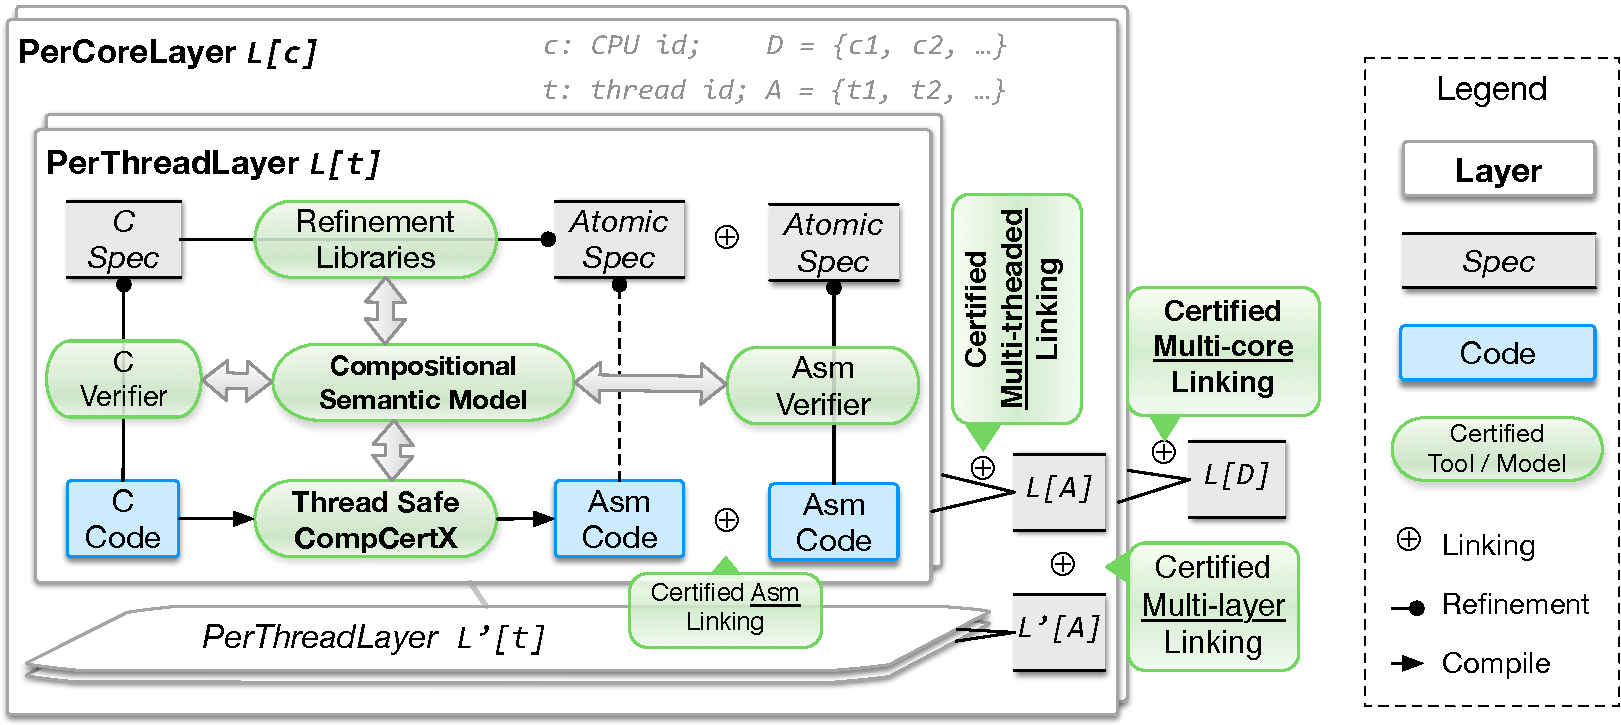
\includegraphics[scale=.45]{figs/tool_chain}
\caption{System architecture of the CCAL programming toolkit.}
\label{fig:toolchain}
\end{figure*}

\begin{table}
\begin{center}
\begin{footnotesize}
\renewcommand{\arraystretch}{1} 
\begin{tabular}{|c|c||c|c|}
\hline
Component & LOC & Component & LOC \\
\hline
\hline
Auxiliary library & 6,200 & Multilayer linking & 17,000 \\
\hline
C verifier & 2,200 & Multithread linking & 10,000 \\
\hline
Asm verifier & 800 & Multicore linking & 7,000 \\
\hline
Simulation library & 1,800 & Thread-safe CompCertX & 7,500\\
\hline
\end{tabular}
\end{footnotesize}
\end{center}
\caption{Lines of proofs in Coq for the toolkit.}
%\hrulefill
\label{table:toolkit}
\end{table}

We have implemented the CCAL toolkit (see Fig. \ref{fig:toolchain}) in the Coq proof assistant. 
Table
\ref{table:toolkit} presents the number of lines (in Coq) for each component in Fig.~\ref{fig:toolchain}. The auxiliary library contains the common
tactics and lemmas for 64 bit integers, lists, maps, integer
arithmetic, {etc}.

\begin{table}
\begin{center}
\renewcommand{\arraystretch}{1.1}
\setlength{\tabcolsep}{0.3em}
\begin{tabular}{|c|c|c|c|c|c|c|}
\hline
 & \makecell{ C \& Asm \\Source} & Specification & \makecell{Invariant \\ Proof} & \makecell{C \& Asm \\Proof} & \makecell{Simulation \\ Proof} \\
%\cline{3-4}
% & Source & Specification & Invariant Proof & Proof & Proof  \\
\hline
Ticket lock & 74 & 615 & 1,080 & 1,173 & 2,296 \\
\hline
MCS lock & 287 & 1,569 & 2,299  &  1,899 & 3,049 \\
\hline
Sequential queue & 377 & 554 & 748 & 2,821& 3,647 \\
\hline
Shared queue &  20 & 107 & 190 & 171& 419\\
\hline
Yield/Sleep/Wakeup & 62 & 153 & 166 & 1,724 & 2,042 \\
\hline
Queuing lock & 112 & 255 & 992 & 328 & 464\\
\hline
\end{tabular}
\newline
\end{center}
\begin{flushright}
* Starvation proof for Ticket lock included: 980\\
** Starvation proof for MCS lock included: 2,455
\end{flushright}
\caption{Statistics for implemented components.}
\label{table:evaluation}
\hrulefill
\end{table}

\para{Case Studies}

To evaluate the framework itself, we have implemented, specified, and verified various
concurrent programs in the framework. Table \ref{table:evaluation} presents some of the
statistics with respect to the implemented components.
As for lock implementations,
their source code contains not only
the code of the associated functions,
but also the data structures and their initialization.
In addition to the top-level interface, the specification contains all the 
specifications used in the intermediate layers.
For both the ticket and MCS locks,
the simulation proof column
includes the proof of starvation freedom (about 1,500 lines) in addition to the correctness proof.
The gap between the underlying C implementation and the high-level specification of the locks
also contributes to the large proof size for these components.
For example, intermediate specification of the ticket lock uses an unbounded
integer for the ticket field,
while the implementation uses a binary integer
which wraps back to zero.
Similarly, the queue is represented as a logical list in the specification,
while it is implemented as a doubly linked list.

Our development is compositional. Both ticket  and MCS locks share the same
high-level atomic specifications.
Thus the lock implementations can be freely interchanged without affecting any proof
in the higher-level modules using locks. When implementing the shared queue library, we
also reuse the implementation and proof of the sequential queue library:
to implement the atomic queue object, we simply wrap the
sequential queue operations with lock acquire and release statements.
As shown in Table \ref{table:evaluation}, using verified lock modules to build
atomic objects such as shared queues is relatively simple and does not require
many lines of code.

Following the same philosophy, 
we have further extended our work with paging-based
dynamically allocated virtual
memory, device drivers with in-kernel interrupts, a synchronous inter-process
communication (IPC) protocol using the queuing lock, a shared-memory IPC protocol with
a shared page, and Intel hardware virtualization support.
We have used the toolkit to produce the world's
first fully certified concurrent OS kernel
with fine-grained locking. 
The entire kernel contains 6,500 lines
of C and x86 assembly code.


\ignore{
To evaluate the framework itself, we have implemented, specified, and verified various
concurrent programs in the framework. Table \ref{table:evaluation} presents some of the
statistics with respect to the implemented components.
\ignore{ in terms of the number of lines of C \& assembly
source code, the number of layers used to specify and verify the module, the size of the
specification, and the number of lines
(in Coq) used to perform the invariant proof, code proof, and refinement proof, respectively.}
\ignore{The largest component is a thread linking refinement component. 
The LoC of multithread linking in Tab.~\ref{table:toolkit} only counts  
generic toolkit files. 
Instantiating them with our actual layer interface definitions which are described in 
Sect.~\ref{sec:multithreaded-layers} requires the refinement of the whole primitives 
in $\Lbthread[i]$ on CompCertX
and $\Lhthread[i][j]$ on Thread-safe CompCertX.
Therefore, the proof heavily relies on the size of layer interfaces.
In this sense, the proof size becomes big in our example because
$\Lbthread[i]$ or $\Lhthread[i][j]$ contains around 70 primitives, 
However, their proofs have redundant parts that can be further optimized 
and automated in the future.}

Lock implementations are  big parts in our examples. 
The first reason or this large LoC is the subtlety of busy waiting in the lock implementation 
(line 14 in Fig.~\ref{fig:exp:ticket_lock_example}). This requires us a large number of proofs to show 
 this loop
terminates within a bound (\ie, starvation-freedom). 
The other reason is mainly related to the strategy simulation 
that we have explained in Sec.~\ref{sec:informal}. 
Since our main goal is facilitating our toolkit for a large concurrent software system 
with scalability,  we have to make sure the the spinlock module provides
a general and simple interface.
This requires us to lift the low-level strategies (or specifications)
of two lock implementation to the same atomic interface (see Sec.~\ref{sec:informal}), which make proofs big.
Despite of this large LoC, however, the client of spinlocks can be verified over a simple interface
thanks to our toolkit.
\jieung{Will reduce and refine this paragraph again.}

\ignore{Their source code contains not only
the code of the associated functions,
but also the data structures and their initialization.
In addition to the top level interface, the specification contains all the 
specifications used in the intermediate layers.
For both the ticket and MCS locks,
the refinement proof column
includes the proof of starvation freedom (about 3,500 lines) in addition to the correctness proof.
The gap between the underlying C implementation and the high level specification of the locks
also contributes to the large proof size for these components.
For example, the intermediate specification of the ticket lock uses an unbounded
integer for the ticket field,
while the implementation uses a binary integer
which wraps back to zero.
Similarly, the queue is represented as a logical list in the specification,
while it is implemented as a doubly linked list.}

In addition to that, Our development is modular. 
Both ticket and MCS locks have the same
abstract specification,
thus the lock implementations can be freely interchanged without affecting any proof
in the higher-level modules using locks. When implementing the shared queue library, we
also reuse the implementation and proof of the sequential queue library:
to implement the atomic queue object, we simply wrap the
sequential queue operations with lock acquire and release.
As shown in Table \ref{table:evaluation}, using verified lock modules to build
atomic objects such as shared queues is relatively simple and does not require
many lines of code.
In addition, we can reuse the same lock verifications and specifications to verify other shared 
objects including a page allocation table.
In this sense, the large number in two lock components are reasonable trade-off
with all the benefits of our toolkits. 

Following the same philosophy, \citet{certikos-osdi16} has
further extended our work with paging-based dynamically allocated
virtual memory, device drivers with in-kernel interrupts, a
synchronous inter-process communication (IPC) protocol using the
queuing lock, a shared-memory IPC protocol with a shared page, and
Intel hardware virtualization support for simultaneously running
multiple virtual machines (one on each core); our CCAL toolkit was
used to produce the world's first fully certified concurrent OS kernel
with fine-grained locking.
\ignore{The entire kernel is reported to contain 6,500 lines
of C and x86 assembly code, and the verification effort for the concurrent kernel
is reported to be 2 person years.} }

\para{Performance Evaluation} 
The verification should not by any means hinder the performance.
One benefit of the layered approach is that
concrete and highly optimized (and thus complex) implementations can be abstracted
into much simpler logical specifications that are easier to reason about.
In our toolkit, the verified source code (both C and assembly) are encoded as
abstract syntax trees in Coq, while CompCertX is written directly in
Coq. We then use Coq's extraction mechanism to produce a program which
compiles the C source code and outputs a single piece of assembly code
for the system. The resulting code is efficient.
We have measured the performance
of the ticket lock on an Intel 4-Core i7-2600S (2.8GHz) processor with 16GB memory.
Initially, the ticket lock implementation incurred a latency of 87 CPU cycles in the
single core case.
After a short investigation, we found that we forgot to remove some function calls
to ``logical primitives'' used for manipulating ghost abstract states. After we removed
these extra null calls, the latency dropped down to only 35 CPU cycles.
%%%
We have also benchmarked the performance of various aspect of verified concurrent kernel,
by comparing it with the big-kernel-lock implementation, and comparing its hypervisor
performance with that of KVM \cite{Gu:2016}.
